%!TEX TS-program = xelatex
\documentclass[12pt, a4paper, oneside]{article}

% Можно вставить разную преамбулу
% пакеты для математики
\usepackage{amsmath,amsfonts,amssymb,amsthm,mathtools}  
\mathtoolsset{showonlyrefs=true}  % Показывать номера только у тех формул, на которые есть \eqref{} в тексте.

\usepackage[british,russian]{babel} % выбор языка для документа
\usepackage[utf8]{inputenc}          % utf8 кодировка

% Основные шрифты 
\usepackage{fontspec}         
\setmainfont{Linux Libertine O}  % задаёт основной шрифт документа

% Математические шрифты 
\usepackage{unicode-math}     
\setmathfont[math-style=upright]{euler.otf} 

\setmathfont[range={\mathbb, \mathop, \heartsuit, \angle, \smile, \varheartsuit}]{Asana-Math.otf}

%%%%%%%%%% Работа с картинками и таблицами %%%%%%%%%%
\usepackage{graphicx} % Для вставки рисунков                
\usepackage{graphics}
\graphicspath{{images/}{pictures/}}   % папки с картинками

\usepackage[figurename=Картинка]{caption}

\usepackage{wrapfig}    % обтекание рисунков и таблиц текстом

\usepackage{booktabs}   % таблицы как в годных книгах
\usepackage{tabularx}   % новые типы колонок
\usepackage{tabulary}   % и ещё новые типы колонок
\usepackage{float}      % возможность позиционировать объекты в нужном месте
\renewcommand{\arraystretch}{1.2}  % больше расстояние между строками


%%%%%%%%%% Графики и рисование %%%%%%%%%%
\usepackage{tikz, pgfplots}  % языки для графики
%\pgfplotsset{compat=1.16}

\usepackage{todonotes} % для вставки в документ заметок о том, что осталось сделать
% \todo{Здесь надо коэффициенты исправить}
% \missingfigure{Здесь будет Последний день Помпеи}
% \listoftodos --- печатает все поставленные \todo'шки

\usepackage{multicol}

%%%%%%%%%% Внешний вид страницы %%%%%%%%%%

\usepackage[paper=a4paper, top=20mm, bottom=15mm,left=20mm,right=15mm]{geometry}
\usepackage{indentfirst}    % установка отступа в первом абзаце главы

\usepackage{setspace}
\setstretch{1.15}  % межстрочный интервал
\setlength{\parskip}{4mm}   % Расстояние между абзацами
% Разные длины в LaTeX: https://en.wikibooks.org/wiki/LaTeX/Lengths

% свешиваем пунктуацию
% теперь знаки пунктуации могут вылезать за правую границу текста, при этом текст выглядит ровнее
\usepackage{microtype}

% \flushbottom                            % Эта команда заставляет LaTeX чуть растягивать строки, чтобы получить идеально прямоугольную страницу
\righthyphenmin=2                       % Разрешение переноса двух и более символов
\widowpenalty=300                     % Небольшое наказание за вдовствующую строку (одна строка абзаца на этой странице, остальное --- на следующей)
\clubpenalty=3000                     % Приличное наказание за сиротствующую строку (омерзительно висящая одинокая строка в начале страницы)
\tolerance=10000     % Ещё какое-то наказание.

% мои цвета https://www.artlebedev.ru/colors/
\definecolor{titleblue}{rgb}{0.2,0.4,0.6} 
\definecolor{blue}{rgb}{0.2,0.4,0.6} 
%\definecolor{red}{rgb}{1,0,0.2} 
\definecolor{green}{rgb}{0, 0.6, 0}
\definecolor{purp}{rgb}{0.4,0,0.8} 

\definecolor{red}{RGB}{213,94,0}
\definecolor{yellow}{RGB}{240,228,66}


% цвета из geogebra 
\definecolor{litebrown}{rgb}{0.6,0.2,0}
\definecolor{darkbrown}{rgb}{0.75,0.75,0.75}

% Гиперссылки
\usepackage{xcolor}   % разные цвета

\usepackage{hyperref}
\hypersetup{
	unicode=true,           % позволяет использовать юникодные символы
	colorlinks=true,       	% true - цветные ссылки
	urlcolor=blue,          % цвет ссылки на url
	linkcolor=black,          % внутренние ссылки
	citecolor=green,        % на библиографию
	breaklinks              % если ссылка не умещается в одну строку, разбивать её на две части?
}

% меняю оформление секций 
\usepackage{titlesec}
\usepackage{sectsty}

% меняю цвет на синий
\sectionfont{\color{titleblue}}
\subsectionfont{\color{titleblue}}

% кружочки у цифр в секциях
\renewcommand{\thesection}{\arabic{section}}

% https://ru.overleaf.com/learn/latex/Sections_and_chapters

% выбрасываю нумерацию страниц и колонтитулы 
%\pagestyle{empty}

% синие круглые бульпоинты в списках itemize 
\usepackage{enumitem}

\definecolor{itemizeblue}{rgb}{0, 0.45, 0.70}

\newcommand*{\MyPoint}{\tikz \draw [baseline, fill=itemizeblue, draw=blue] circle (2.5pt);}
\renewcommand{\labelitemi}{\MyPoint}

\AddEnumerateCounter{\asbuk}{\@asbuk}{\cyrm}
\renewcommand{\theenumi}{\asbuk{enumi}}

% расстояние в списках
\setlist[itemize]{parsep=0.4em,itemsep=0em,topsep=0ex}
\setlist[enumerate]{parsep=0.4em,itemsep=0em,topsep=0ex}

% эпиграфы
\usepackage{epigraph}
\setlength\epigraphwidth{.6\textwidth}
\setlength\epigraphrule{0pt}

%%%%%%%%%% Свои команды %%%%%%%%%%

% Математические операторы первой необходимости:
\DeclareMathOperator{\sgn}{sign}
\DeclareMathOperator*{\argmin}{arg\,min}
\DeclareMathOperator*{\argmax}{arg\,max}
\DeclareMathOperator{\Cov}{Cov}
\DeclareMathOperator{\Var}{Var}
\DeclareMathOperator{\Corr}{Corr}

\DeclareMathOperator{\Pois}{Pois}
\DeclareMathOperator{\Geom}{Geom}
\DeclareMathOperator{\Exp}{Exp}

%\DeclareMathOperator{\E}{\mathbb{E}}
\DeclareMathOperator{\Med}{Med}
\DeclareMathOperator{\Mod}{Mod}
\DeclareMathOperator*{\plim}{plim}

% команды пореже
\newcommand{\const}{\mathrm{const}}  % const прямым начертанием
\newcommand{\iid}{\sim i\,i\,d\,\,}  % ну вы поняли...
\newcommand{\fr}[2]{\ensuremath{^{#1}/_{#2}}}   % особая дробь
\newcommand{\ind}[1]{\mathbbm{1}_{\{#1\}}} % Индикатор события
\newcommand{\dx}[1]{\,\mathrm{d}#1} % для интеграла: маленький отступ и прямая d

% одеваем шапки на частые штуки
\def \hb{\hat{\beta}}
\def \hs{\hat{s}}
\def \hy{\hat{y}}
\def \hY{\hat{Y}}
\def \he{\hat{\varepsilon}}
\def \hVar{\widehat{\Var}}
\def \hCorr{\widehat{\Corr}}
\def \hCov{\widehat{\Cov}}

% Греческие буквы
\def \a{\alpha}
\def \b{\beta}
\def \t{\tau}
\def \dt{\delta}
\def \e{\varepsilon}
\def \ga{\gamma}
\def \kp{\varkappa}
\def \la{\lambda}
\def \sg{\sigma}
\def \tt{\theta}
\def \Dt{\Delta}
\def \La{\Lambda}
\def \Sg{\Sigma}
\def \Tt{\Theta}
\def \Om{\Omega}
\def \om{\omega}

% Готика
\def \mA{\mathcal{A}}
\def \mB{\mathcal{B}}
\def \mC{\mathcal{C}}
\def \mE{\mathcal{E}}
\def \mF{\mathcal{F}}
\def \mH{\mathcal{H}}
\def \mL{\mathcal{L}}
\def \mN{\mathcal{N}}
\def \mU{\mathcal{U}}
\def \mV{\mathcal{V}}
\def \mW{\mathcal{W}}

% Жирные буквы
\def \mbb{\mathbb}
\def \RR{\mbb R}
\def \NN{\mbb N}
\def \ZZ{\mbb Z}
\def \PP{\mbb{P}}
\def \E{\mbb{E}}
\def \QQ{\mbb Q}

\def\F{\ensuremath{\mathcal{F}}} % аналогично!

%%%%%%%%%% Теоремы %%%%%%%%%%
\theoremstyle{plain} % Это стиль по умолчанию.  Есть другие стили.
\newtheorem{theorem}{Теорема}[section]
\newtheorem{proposition}{Утверждение}[section]
\newtheorem{result}{Следствие}[section]

% убирает курсив и что-то еще наверное делает ;)
\theoremstyle{definition}         
\newtheorem*{definition}{Определение}  % нумерация не идёт вообще


%%%%%%%%%% Задачки и решения %%%%%%%%%%
\usepackage{etoolbox}    % логические операторы для своих макросов
\usepackage{environ}
\newtoggle{lecture}

\newcounter{probNum}[section]  % счётчик для упражнений 
\NewEnviron{problem}[1]{%
    \refstepcounter{probNum}% увеличели номер на 1 
    {\noindent \textbf{\large \color{titleblue} Упражнение~\theprobNum~#1}  \\ \\ \BODY}
    {}%
  }

% Окружение, чтобы можно было убирать решения из pdf
\NewEnviron{sol}{%
  \iftoggle{lecture}
    {\noindent \textbf{\large Решение:} \\ \\ \BODY}
    {}%
  }
 
% выделение по тексту важных вещей
\newcommand{\indef}[1]{\textbf{ \color{green} #1}} 

% разные дополнения для картинок
\usetikzlibrary{arrows.meta}
\usepackage{varwidth}

\usepackage[normalem]{ulem}  % для зачекивания текста

% Если переключить в false, все solution исчезнут из pdf
\toggletrue{lecture}
%\togglefalse{lecture}



\title{
\begin{center} 
\includegraphics[width=0.99\textwidth]{logo.png}
\end{center}

Посиделка 6: сходимости случайных величин}
\date{ } %\today}

% Если делаешь конспект, вписывай своё имя прямо сюда!
\author{Ульянкин Ппилиф}

\begin{document} % Конец преамбулы, начало файла

\maketitle

\epigraph{Повторять до сходимости --- это как жарить до готовности.}{\textit{(Неизвестный студент Вышки)}}

В этой посиделке мы поговорим про сходимости, которые часто встречаются в теории вероятностей и математической статистике. Не очень понятно, нафига придумывать какие-то новые сходимости, когда в матане мы уже изучили сходимость обычных последовательностей. Попробуем с этим разобраться. 

% \todo[inline]{Для всех сходимостей расписать свойства без доказательств. Перепридумать разделы с союзниками и зачемами.}

\section{Обычная сходимость}

Говорят, что последовательность действительных чисел $(a_n)_{n=1}^{\infty}$ сходится к числу $A$ т.е.

\[ 
\lim_{n \to \infty} a_n = A,
\]

если для любого сколь угодно малого положительного числа $\varepsilon > 0$ существует порядковый номер $N(\varepsilon) \in \NN$ такой, что начиная с него $a_n$ отличается от $A$ меньше чем на $\varepsilon$ т.е. 

\[
\forall \varepsilon > 0 \quad  \exists N(\varepsilon) \in \NN : \quad  \forall n > N(\varepsilon) \quad |a_n - A| < \varepsilon.
\]

Рассмотрим конкретный пример. Возьмём последовательность $a_n = 10 \cdot n^{0.99} \cdot \sin(n) + \pi.$ Она сходится. Причём к числу $\pi$. Отложим по оси $x$ номера членов последовательности, а по оси $y$ значения. 

\begin{center} 
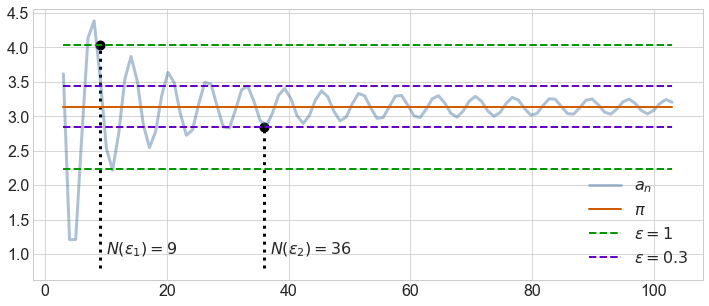
\includegraphics[width=0.95\linewidth]{simple_seq.png}
\end{center} 

Зафиксируем произвольное число $\varepsilon$, например $1$. Начиная с $N(\varepsilon) = 9$ все члены последовательности оказываются зажаты зелёной окрестностью. 

Если взять $\varepsilon = 0.3$, то $N(\varepsilon)$ сдвинется вправо и окажется равно $36$. Если мы для каждого $\varepsilon$ можем найти место, начиная с которого все члены последовательности лежат внутри выделенного нами коридора, то последовательность сходится.

Так обстоят дела с детерминированными последовательностями. В случае, когда речь идёт о последовательностях из случайных величин, всё оказывается немного сложнее. Случайные величины могут с лёгкостью пробивать построенный нами коридор из эпсилонов в любом месте. Из-за этого приходится формулировать сходимость в терминах вероятностей. 

Всего в теории вероятностей выделяют четыре вида сходимости. На картинке ниже стрелками показано, какая сходимость следует из какой. 

\begin{center} 
\begin{tikzpicture}
\node[draw,rectangle,inner sep=5pt] (prob) at (2,-1) {$X_n \overset{p}{\to} X$};
\node[draw,rectangle,inner sep=5pt] (dist) at (5,-1) {$X_n \overset{d}{\to} X$};
\node[draw,rectangle,inner sep=5pt] (alsh) at (-1,0) {$X_n \overset{a.s.}{\to} X$};
\node[draw,rectangle,inner sep=5pt] (mean) at (-1,-2) {$X_n \overset{L^{r}}{\to} X$};

\draw[->,very thick] (prob) -- (dist);
\draw[->,very thick] (alsh) -- (prob);
\draw[->,very thick] (mean) -- (prob);
\end{tikzpicture}
\end{center} 

\begin{itemize} 
\item Самая слабая сходимость, \indef{сходимость по распределению.} Чтобы сказать, что последовательность случайных величин $X_n$ сходится по распределению к случайной величине $X$, обычно над стрелочкой пишут букву $L$ или букву $d$. Иногда просто рисуют двойную стрелочку, $\Rightarrow$. Из-за того, что эта сходимость самая слабая её так иногда и называют --- \indef{слабой сходимостью.}

\item Сходимость чуть посильнее --- это \indef{сходимость по вероятности.} Обычно её обозначают, подписывая над стрелкой букву $p$. Если последовательность сходится по вероятности, тогда она будет сходиться и по распределению. 

\item Сходимость по вероятности, в свою очередь следует из \indef{сходимости почти наверное.} (almost surely). Чтобы обозначить эту сходимость, над стрелкой пишут $a.s.$ или п.н. Эту сходимость часто называют \indef{сильной сходимостью.} 

\item Также сходимость по вероятности следует из \indef{сходимости в среднем порядка $r$.} Над стрелкой в случае такой сходимости либо подписывают порядок сходимости, либо пишут $L^r$. В случае, когда $r=1$ говорят о \indef{сходимости в среднем.} В случае $r=2$ говорят о сходимости \indef{в смысле среднего квадратического.}
\end{itemize} 

Последние два вида сходимости самые сильные. Между ними нет чёткой взаимосвязи. Давайте посмотрим по очереди на все четыре вида. Начнём со сходимости по вероятности. 


\section{Сходимость по вероятности}

\begin{definition} 
Последовательность случайных величин $X_1, X_2, X_3, \ldots$ \indef{сходится по вероятности} к случайной величине $X$, если 
\[
\forall \varepsilon > 0 \quad \lim_{n \to \infty} \PP(|X_n - X| > \varepsilon) = 0.
\]

Обычно это записывают, как $X_n \overset{p}{\to} X$, либо $\plim\limits_{n \to \infty} X_n = X$.
\end{definition} 

Довольно часть сходимость по вероятности можно доказать просто воспользовавшись определением.  

\begin{problem}{ } 
Пусть $X_n \sim Exp(n)$. Покажите, что $X_n \overset{p}{\to} 0$.
\end{problem} 

\begin{sol}
Пойдём чётко по определению
\[
\lim_{n \to \infty} \PP(|X_n - X| > \varepsilon) = \lim_{n \to \infty} \PP(X_n > \varepsilon).
\]

Воспользуемся определением функции распределения: $\PP(X_n > \varepsilon) = 1 - \PP(X_n \le \varepsilon)$.
\[
\lim_{n \to \infty} \PP(X_n > \varepsilon) = \lim_{n \to \infty} 1 - (1 - e^{-n \varepsilon}) = \lim_{n \to \infty}  e^{-n \varepsilon} = 0 \quad \forall \varepsilon > 0.
\]

Получается, что 

\[
\plim_{n \to \infty} X_n = 0.
\]

Подумайте, что будет для $X_n \sim Exp\left( \frac{1}{n} \right)$.
\end{sol}

\subsection{Сходимость по вероятности в картинках}

Для обычной сходимости нам было нужно, чтобы начиная с какого-то номера $N(\varepsilon)$ вся последовательность оставалась в рамках коридора из эпсилонов. В случае сходимости по вероятности, когда мы оказываемся за некоторым номером $N(\varepsilon)$, последовательность может пробивать коридор. Но по мере нашего продвижения вправо, вероятность того, что она пробьёт коридор падает. 

Давайте попробуем посмотреть на это на конкретном примере. Предположим, что в наших руках оказалась генеральная совокупность из нормального распределения. Мы сделали из неё выборку некоторого объёма и посчитали по ней выборочное среднее. 

$$
\bar X = \sum_{i=1}^n X_i
$$

Выборочное среднее сходится по вероятности к математическому ожиданию при росте  $n$. Этот факт обычно называют законом больших чисел. В следующей посиделке мы сформулируем его как полноценную теорему. Тут же давайте посмотрим как это выглядит в картинках

\begin{center} 
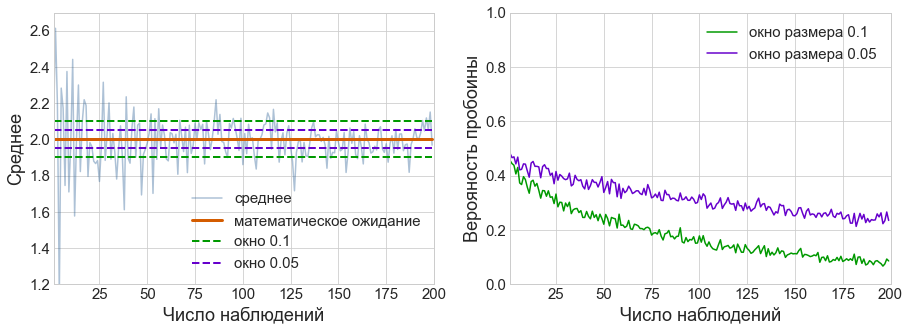
\includegraphics[width=0.99\linewidth]{plim_2.png}
\end{center} 

Зафиксируем коридор, $\varepsilon$, за которым мы будем в дальнейшем наблюдать. Как можно увидеть, поначалу, при маленьком числе наблюдений, последовательность довольно часто пробивает коридор. Нет такого, чтобы она один раз погрузилась в него и никогда больше из него не выходила. Со временем, количество пробоин в зафиксированном коридоре падает.

Можно попробовать оценить вероятность того, что последовательность из средних пробьёт на конкретном шаге установленный нами коридор. Для этого можно сгенерировать $1000$ траекторий среднего, а дальше посмотреть, как часто на каждом шаге у нас возникает пробоина. Частота таких пробоин и будет оценкой вероятности пробить коридор. Именно её динамика для обоих наших коридоров нарисована на картинке справа. 

Теперь мы знаем, как выглядит сходимость по вероятности. Интересно было бы посмотреть, как выглядит её отсутствие. Давайте вспомним распределение Коши. У него не существует математического ожидания и для него выборочному среднему некуда сходиться. Давайте построим для него пару таких же рисунков. 

Мы видим, что среднее постоянно пробивает выделенный нами коридор. При этом, с ростом $n$, число пробоин не уменьшается. Вероятность пробоины не убывает и ведёт себя стабильно. 

\begin{center} 
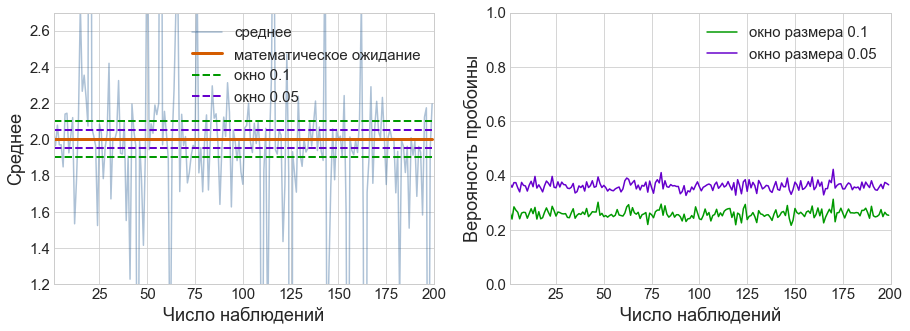
\includegraphics[width=0.99\linewidth]{plim_3.png}
\end{center} 


\subsection{Друзья сходимости по вероятности}

У сходимости по вероятности есть много друзей, которые помогают проверять её наличие. 

\begin{itemize} 
\item Первый и главный друг сходимости по вероятности --- это закон больших чисел. 

\begin{theorem}{\textbf{Закон Больших Чисел (Пафнутий Львович Чебышёв)}}

Пусть $X_1, \ldots, X_n$ попарно независимые и одинаково распределённые случайные величины с конечным вторым моментом, $E(X_i^2) < \infty$, тогда имеет место сходимость:

$$
\frac{X_1 + \ldots + X_n}{n} \overset{p}{\to} E(X_1)
$$
\end{theorem}

Про него мы подробно поговорим в следующей посиделке.

\item Второй друг сходимости по вероятности --- неравенства Чебышёва и Маркова. Они иногда помогают доказать наличие сходимости по определению.

\begin{theorem}
Если у случайной величины $X$ конечная дисперсия, тогда $\forall \varepsilon > 0$

$$
\PP(|X| \ge \varepsilon) \le \frac{\E(X)}{\varepsilon}
$$

А также 

$$
\PP(|X - \E(X)| \ge \varepsilon) \le \frac{\Var(X)}{\varepsilon^2}.
$$
\end{theorem}

Чтобы запомнить, где какие неравенства ставить, можно представить себе что-то подозревающего китайца\footnote{Эта рукопись может содержать устаревшие культурные стереотипы и показывается в оригинальном виде}. 

\begin{center} 
\begin{tikzpicture}
\draw (0,0) ellipse (1.2cm and 0.8cm);
\node at (0.4,0.2) {$\le$};
\node at (-0.4,0.2) {$\ge$};
\node at (0,-0.1) {$\angle$};
\node at (0,-0.5) {$\smile$};
\end{tikzpicture}
\end{center} 

В упражнении, которое мы решали выше, неравенством Маркова можно было бы воспользоваться следующим образом

\[
\PP(X_n \ge \varepsilon) \le \frac{\E(X)}{\varepsilon} = \frac{1}{n \cdot \varepsilon} \to 0, \text{ при } n \to \infty.
\]

Получается искомая нами вероятность ограничена при $n \to \infty$ сверху нулём. Получается она будет равна нулю. 

\item Третий друг --- это арифметические свойства предела. Из-за того, что сходимость по вероятности --- наследник обычной сходимости, все свойства сохраняются~\cite{ref:chern}. 

\item Четвёртый союзник --- это теорема Манна-Вальда. В русской литературе её часто называют теоремой Слуцкого. На самом деле в сходимостях есть ещё одна теорема Слуцкого, которую мы будем обсуждать немного ниже. Чтобы не запутаться, будем называть эту теорему на западный манер\footnote{Запад развращает. Сначала ты начинаешь писать вместо $M$ букву $\E,$ а затем переименовываешь теоремы.}. 

\begin{theorem}{\textbf{Манна-Вальда-Слуцкого}}

\begin{itemize} 
\item Если $X_n \overset{p}{\to} a$ и функция $g(t)$ непрерывна в точке $a$, тогда $g(X_n) \overset{p}{\to} g(a).$
\item Если $X_n \overset{p}{\to} X$ и функция $g(t)$ непрерывна, тогда $g(X_n) \overset{p}{\to} g(X).$
\end{itemize} 
\end{theorem}

Доказательство этой теоремы и ещё ряда свойств можно найти, например, в книге Черновой~\cite{ref:chern}.
\end{itemize} 

\subsection{Зачем всё это, зачем?}

Нам это всё нужно для благих целей. Чаще всего сходимость по вероятности будет нам требоваться для доказательства состоятельности. Когда мы собираем выборку для того, чтобы оценить какой-нибудь параметр, мы надеемся, что из-за её больших размеров мы окажемся близко к истине. Состоятельность говорит нам именно про это. 

\begin{definition} 
Оценка $\hat \theta$ неизвестного параметра $\theta$ называется \indef{состоятельной,} если при $n \to \infty$ она сходится по вероятности к истинному значению, то есть $\hat \theta  \overset{p}{\to} \theta$. 
\end{definition}

В будущих посиделках мы будем доказывать состоятельность разных оценок, используя перечисленных выше союзников. 


\section{Сходимость по распределению}

\begin{definition} 
Последовательность случайных величин $X_1, X_2, X_3, \ldots$ \indef{сходится по распределению} к случайной величине $X$, если при $n \to \infty$ последовательность $F_{X_n}(x) \to F_X(x)$ для всех $x$, в которых $F_X(x)$ непрерывна. Обычно это записывают, как $X_n \overset{d}{\to} X$ либо $X_n \Rightarrow X$. Ещё \indef{такую сходимость называют слабой,} так как она следует из всех остальных сходимостей. 
\end{definition}

\subsection{Сходимость по распределению в картинках}

Если последовательность из функций сходится, она есть. Если не сходятся, её нет. Всё просто. 

\begin{problem}{ } 
Пусть последовательность $X_1, X_2, \ldots $ это последовательность случайных величин с функциями распределения 

$$
F_{X_n}(x) = \begin{cases} 1 - \left(1 - \frac{1}{n} \right)^{nx} \quad& x \ge 0 \\ 0 \quad & \text{иначе} \end{cases}
$$

Найдите предел по распределению для $X_n$. 
\end{problem} 

\begin{sol}
Надо просто найти предел для $F_{X_n}(x)$: 

$$
F_X(x) = \lim_{n \to \infty} F_{X_n}(x) = 1 - e^{-x}.
$$

Получаем в пределе экспоненциальное распределение, $Exp(1)$. 
\end{sol}

Другой пример, который часто встречается на практике --- распределение Стьюдента с $n$ степенями свободы, $t(n)$. Оно славится тем, что обладает более тяжёлыми хвостами, чем у нормального распределения. При этом, если $n \to \infty$, распределение Стьюдента сходится по распределению к стандартному нормальному, $t(n) \overset{d}{\to} N(0,1).$ 

Можно проиллюстрировать этот факт на картинке. Чёрная пунктирная линия --- стандартное нормальное распределение. Остальные линии это распределённые по стьюденту случайные величины. Видно, что и плотности и функции распределения понемногу приближаются к предельной. 

\begin{center} 
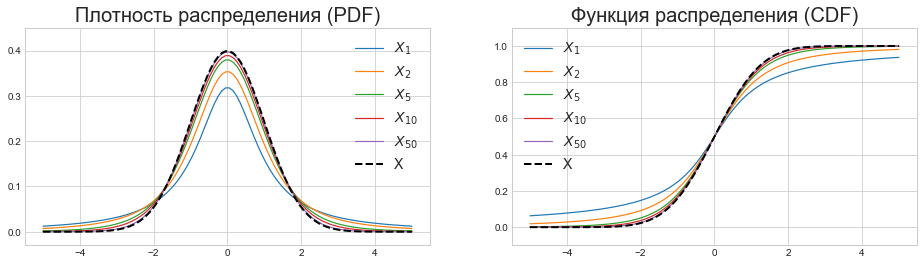
\includegraphics[width=0.99\linewidth]{student.png}
\end{center} 

Можно выписать функцию плотности для распределения Стьюдента и осознать как именно так получается, но мы оставим это читателю в качестве домашнего задания. В определении не очень понятной остаётся формулировка <<для всех $x$, в которых $F_X(x)$ непрерывна.>> Чтобы лучше понять её, давайте решим ещё одну задачку.

\begin{problem}{ } 
Пусть $X_n \sim U[0;1],$ а $Y_n = \min(X_1, \ldots, X_n).$ Найдите $F_{Y_n}(y)$, а затем докажите, что $Y_n \overset{d}{\to} 0$ и что  $Y_n \overset{p}{\to} 0.$
\end{problem} 

\begin{sol}
Для начала найдём функцию распределения минимума из $n$ независимых случайных величин 

\begin{multline*} 
F_{Y_n}(y) = \PP(Y_n \le y) = \PP(\min(X_1, X_2, \ldots, X_n) \le y) = 1 - \PP(\min(X_1, X_2, \ldots, X_n) > y).
\end{multline*} 

Если минимум больше $y$, то и все случайные величины должны быть больше него

\begin{multline*} 
F_{Y_n}(y) = 1 - \PP(X_1 > y, X_2 > y, \ldots, X_n > y) = \\ = 1 - \PP(X_1 > y) \cdot \PP(X_2 > y) \cdot \ldots \cdot \PP(X_n > y) = \\ = 1 - [1 - \PP(X_1 \le y)] \cdot [1 - \PP(X_2 \le y)] \cdot \ldots \cdot [1 - \PP(X_n \le y)] = \\ = 1 - [1 - F_{X_n}(y)]^n = 1 - [1 - y]^n.
\end{multline*} 

Получается, что 

\begin{equation*} 
F_{Y_n}(y) = \begin{cases}0, \text{ если } y < 0 \\ 1, \text{ если } y \ge 1 \\ 1 - [1 - y]^n, \text{ если } y \in [0; 1).    \end{cases}
\end{equation*}

Докажем, что $Y_n \overset{d}{\to} 0.$ Функция распределения вырожденной случайной величины, принимающей только значение $1$ выглядит как 

\begin{equation*} 
F_{Y}(y) = \begin{cases}1, \text{ если } y \ge 0 \\ 0, \text{ если } y < 0 \end{cases}
\end{equation*}

Найдём предел $F_n(y)$ во всех точках $y$ и сравним его с $F(y)$

\begin{equation*} 
\begin{aligned} 
& y \ge 1 \quad F_{Y_n}(y) = 1 \to 1 = F_{Y}(y) \\ 
& y < 0 \quad F_{Y_n}(y) = 0 \to 0 = F_{Y}(y) \\ 
& 0 < y < 1 \quad F_{Y_n}(y) = 1 - [1 - y]^n \to 1 = F_{Y}(y) \\ 
& y = 0 \quad F_{Y_n}(y) = 0 \to 0 \ne 1 = F_{Y}(y) \\ 
\end{aligned} 
\end{equation*} 

В точке $y = 0$ сходимости нет. Определение сходимости по распределению разрешает нам проигнорировать эту точку, потому что у предельной функции $F_Y(y)$ в ней есть разрыв. 
\end{sol}

\subsection{Друзья сходимости по распределению}

Доказывать сходимость по распределению проще, чем сходимость по вероятности. Достаточно просто понять, как ведут себя функции распределения. Тем не менее, у сходимости по распределению тоже есть друзья, которыми мы дальше будем пользоваться.

\begin{itemize} 
\item Во-первых, это ЦПТ. 

\begin{theorem}{\textbf{Центральная Предельная Теорема (Прокопий Петрович Ляпунов)}}

Пусть $X_1, \ldots, X_n$ попарно независимые и одинаково распределённые случайные величины с конечным вторым моментом, $E(X_i^2) < \infty$, тогда при $n \to \infty$ имеет место сходимость по распределению: 

$$
\bar{x} \overset{d}{\to} N \left(\E(X_i), \frac{\Var(X_i)}{n} \right)
$$

Этот же факт можно переписать немного иначе:

\[\sqrt{n} \cdot [\bar{x} - \E(X_i)]  \overset{d}{\to} N \left(0, \Var(X_i)\right)\]

или даже как

\[\sqrt{n} \cdot \frac{\bar{x} - \E(X_i)}{\sqrt{\Var(X_i)}}  \overset{d}{\to} N \left(0, 1\right).\]

\end{theorem}

Если говорить простым языком, то при определённых условиях сумма достаточно большого числа случайных величин имеет распределение близкое к нормальному. \indef{Главное, чтобы случайные величины были похожи и не было такого, что одна резко выделяется на фоне остальных.} Разговору о ЦПТ мы посвятим следующую посиделку. 

\item Во-вторых, это обобщение ЦПТ --- Дельта-метод. Его мы введём, когда будем строить статистику средних. 

\item В-третьих, это ещё одна теорема Слуцкого. Она так называется и на Западе. 

\begin{theorem}{\textbf{Слуцкого}}
Если $X_n \overset{p}{\to} a \ne 0$ и $Y_n \overset{d}{\to} Y$, тогда 
\begin{itemize} 
\item $Y_n + X_n \overset{d}{\to} Y + a$
\item $Y_n \cdot X_n \overset{d}{\to} Y \cdot a$
\item $\frac{Y_n}{X_n} \overset{d}{\to} \frac{Y}{a}.$
\end{itemize}
\end{theorem}

\end{itemize} 

Ещё раз подчеркнём, что сходимость по распределению самая слабая. Если есть сходимость по вероятности, то будет и сходимость по распределению. В обратную сторону это верно только в случае сходимости к константе. На доказательство этих замечательных фактов можно, например, в лекциях Дэвида Хантера.~\cite{ref:hanter} Вам нужна будет вторая глава.

\subsection{Зачем всё это, зачем?}

Помните, в самом начале мы говорили про схему матстата? Мы сказали, что когда у нас есть точечная оценка, нам хочется понять, насколько она точная. Для этого надо пытаться выяснить как оценка распределена. Нужен союзник, который подскажет. Сходимость по распределению, в частности ЦПТ, помогает находить асимптотических союзников для этих целей. 


\section{Сходимость в среднем} 

Когда мы придумываем определение для сходимости $X_n$ к $X$, мы обычно придумываем какое-то расстояние между $X$ и $X_n$. Если оно становится всё меньше и меньше, значит последовательность сходится. Если мы определим это расстояние как $\PP(|X_n - X| > \varepsilon),$ тогда мы получим сходимость по вероятности. Другой способ определить расстояние между случайными величинами --- посмотреть на математическое ожидание. 

\begin{definition} 
Последовательность случайных величин $X_1, X_2, X_3, \ldots$ \indef{сходится в среднем порядка $r$} к случайной величине $X$, если 

\[
\lim_{n \to \infty} \E(|X_n - X|^r) = 0.
\]

Обычно это записывают, как $X_n \overset{L^r}{\to} X$ либо $X_n \overset{m.s.}{\to} X$ в случае, когда $r=2$.
\end{definition}

Из этой сходимости следует сходимость по вероятности и сходимость по распределению. При этом её довольно легко проверить. Чаще всего она нужна, как техническое условие в разных теоремах, поэтому мы с ней будем сталкиваться довольно редко. Тем не менее, для полноты картины с этим видом сходимости тоже нужно немного поработать.

\begin{problem}{ } 
Пусть $X_n \sim U \left[ 0;\frac{1}{n} \right]$. Покажите, что $X_n \overset{L^r}{\to} 0$.
\end{problem} 

\begin{sol}
Воспользуемся определением. Плотность распределения для $X_n$ выглядит как 

\[
f_{X_n}(x) = \begin{cases}  n, \quad 0 \le x \le \frac{1}{n} \\ 0, \quad \text{иначе} \end{cases}.
\]

Найдём 

\[
\E(|X_n - 0|^r) = \int_0^{\frac{1}{n}} x^r \cdot n \dx{x} = \frac{1}{(r + 1) n^r} \to 0 \quad \forall r \ge 1.
\]

Выходит, что $X_n \overset{L^r}{\to} X$ при $r \ge 1$. В подобранном примере все $x$ положительные, поэтому проблем с модулем не возникло. 
\end{sol}

Коли у нас есть сходимость в среднем, то остальные две сходимости тоже будут присутствовать. Сходимость по вероятности можно углядеть, если понять, что дисперсия случайной величины $X_n$ с каждым новым $n$ всё меньше. Сходимость по распределению к вырожденному распределению можно углядеть, если заметить, что в плотности распределения фигурирует $1/n$. Точно такое же $1/n$ будет фигурировать в функции распределения и последовательность из них будет сходиться к вырожденному распределению.

\indef{Сходимость по вероятности слабее.} Иногда бывает так, что сходимость по вероятности есть, но сходимости в среднем нет. Пусть последовательность дискретных случайных величин задаётся следующим образом: 

$$
X_n = \begin{cases} n^2, \qquad p = \frac{1}{n} \\ 0, \qquad p = 1 - \frac{1}{n} \end{cases} 
$$

Эта последовательность будет сходиться к нулю по вероятности

$$
\lim_{n \to \infty} P(|X_n - 0| \ge \varepsilon) = \lim_{n \to \infty} P(X_n = n^2) = \lim_{n \to \infty} \frac{1}{n} = 0.
$$

Число $n$ растёт во времени, а $\varepsilon > 0$ произвольное маленькое число. Чтобы разница $X_n - 0$ оказалась больше этого произвольного маленького числа, нужно, чтобы случайная величина приняла значение $n^2$, поэтому $P(|X_n - 0| \ge \varepsilon) = P(X_n = n^2)$.  

При этом, наша последовательность не будет сходиться к нулю в среднем

$$
\lim_{n \to \infty} E(|X_n|^r) = \lim_{n \to \infty} (n^{2r} \cdot \frac{1}{n} + 0 \cdot (1- \frac{1}{n})) = \lim_{n \to \infty} n^{2r - 1} = \infty \qquad \forall r \ge 1.
$$

У сходимости в среднем есть довольно интересное свойство, связанное с моментами.

\begin{proposition}
Пусть $1 \le r \le s$. Если $X_n \overset{L^s}{\to} X,$ тогда $X_n \overset{L^r}{\to} X$.
\end{proposition}

% \begin{proof}
% Воспользуемся неравенством Йенсена: 

% \[
% \E(|XY|) \le (\E(|X|^p))^{\frac{1}{p}} \cdot (\E(|Y|^q))^{\frac{1}{q}}, \quad 1 < p,q < \infty, \quad \frac{1}{p} + \frac{1}{q} = 1.
% \]

% У нас $X =|X_n - X|^r$, $Y = 1$. Возьмём $p = \frac{s}{r} > 1$. Выходит, что 

% \[
% \E(|X_n - X|^r) \le (\E(|X_n -X|^s))^{\frac{1}{p}} \to 0,
% \]

% так как $\E(|X_n -X|^s) \to 0$. Получается, что $X_n \overset{L^r}{\to} X$.
% \end{proof}

Для сходимости в среднем также работает теорема о непрерывном отображении (Манна-Вальда-Слуцкого), то есть если $X_n \overset{L^r}{\to} X$ и функция $g(t)$ непрерывна, тогда $g(X_n) \overset{L^r}{\to} g(X).$



\section{Сходимость почти наверное} 

Осталось разобраться с последним видом сходимости, сходимостью почти наверное. До этого мы с вами никогда не вдавались в то, как именно устроена случайная величина. Для сходимости почти наверное --- это жутко важно. Поэтому немного вспомним основные определения. 

\subsection{Сигма-алгебра} 

\begin{problem}{}
Рассмотрим простой случайный эксперимент: игральный кубик подбрасывают два раза. Множество $\Om$ исходов данного эксперимента содержит $36$ элементов. Вася знает результат подбрасываний, и сообщает Пете значение случайной величины $Z$ --- произведения очков на выпавших гранях.

Всегда ли сможет Петя, владея своей информацией, определить произошли ли события: $A$ --- оба раза выпала единица, $B$ --- хотя бы раз выпала пятерка, $C$ --- хотя бы раз выпала шестерка?
\end{problem} 

\begin{sol} 
Про события $A$ и $B$ Петя всегда сможет сказать произошли ли они: в первом случае достаточно сравнить $Z$ с единицей, во втором --- определить, делится ли $Z$ на 5. Однако может сложиться такая ситуация, что Петя не будет уверен, произошло ли $C$: например, если $Z$ окажется равным шести, то, может быть, это была пара $(6,1)$ и тогда $C$ произошло, а может это была пара $(2,3)$ и тогда $C$ не произошло.

Можно составить список событий, про которые Петя, зная $Z$, всегда сможет сказать, произошли ли они. Обозначим этот список событий буквой $\F$. В отличие от Пети Вася может уверенно сказать произошло ли любое событие и аналогичный список событий для него --- все подмножества множества $\Om$.
\end{sol} 

В список $\F$ входят довольно много событий, а сам список обладает рядом важных свойств, а именно:

\begin{enumerate}
\item  Множество $\Om \in \F$ --- даже ничего не зная, можно быть уверенным, что событие $\Om$ произошло.

\item  Множество $\varnothing \in \mathcal{F}$ --- даже ничего не зная, можно быть уверенным, что событие $\varnothing$ не произошло.

\item  Если множества $A$ и $B$ входят в список $\F$, то $A\cup B$ и $A\cap B$ входят в список $\F$. Если Петя способен определить, произошли ли $A$ и $B$ по отдельности, то он путем простых логических заключений способен определить, произошли ли $A\cup B$ и $A\cap B$.
\end{enumerate}

Подобные списки событий являются очень важными для нас и называются сигма-алгебрами ($\sigma$-алгебрами).

\begin{definition}  Набор подмножеств множества $\Omega$ называется \indef{$\sigma$-алгеброй}, если обладает следующими тремя свойствами:

\begin{enumerate}
\item[SA1] Множество $\Omega \in \mathcal{F}$

\item[SA2] Из того, что множество $A\in \mathcal{F}$ следует, что $A^{c}\in \mathcal{F}$

\item[SA3] Если $A_{1}\in\mathcal{F}$, $A_{2}\in\mathcal{F}$, $A_{3}\in\mathcal{F}$, и т.д., то $\cup_{i=1}^{\infty} A_{i} \in\mathcal{F}$.
\end{enumerate}
\end{definition} 

Сигма-алгебры нужны для того, чтобы моделировать наделенность информацией рационального индивида. Также они нужны для некоторых технических целей в различных теоремах. Сигма-алгебры помогают моделировать ситуации, когда в сознании наблюдателя несколько событий по каким-то причинам «слипаются», и наблюдатель не может отличить их друг от друга. 

\begin{definition}
\indef{Случайная величина} --- это функция, которая отображает сигма-алгебру на множество действительных чисел, $X(\omega) : \F \to \mathbb{R}$.
\end{definition} 

До текущего момента мы не особо вдавались в подробности, связанные с тем как устроена случайная величина $X(\omega)$ при разных значениях $\omega$. Всем сходимостям выше было на это наплевать. Со сходимостью почти наверное другая история. 

\subsection{Сходимость почти наверное} 

Чтобы стало немного полегче понять определение, давайте решим упражнение. Пусть у нас есть монетка, и мы подкидываем её один раз. Пространство элементарных исходов в таком случае выглядит как: $\Omega = \{O, P\}$. Определим последовательность случайных величин следующим образом.

$$
X_n(\omega) = \begin{cases} \frac{n}{n+1}, \qquad \omega = O \\ (-1)^n, \qquad \omega = P \end{cases}
$$

Пусть мы один раз подбрасываем монетку, а затем выписываем последовательность. Для каких $\omega$ последовательность случайных величин сходится? 

Ответ прост. Ежели выпал орёл, то последовательность вошла в траекторию $\frac{n}{n+1}$ и сошлась к единице. Если выпала решка, то всё пропало. Найдём вероятность $$ \PP(\lim_{n \to \infty} X_n(\omega) = 1).$$

Нам нужно найти вероятность события, которое заключается в том, что наша последовательность сойдётся. Очевидно, что такая вероятность равна $0.5$, так как последовательность будет сходиться только при выпадении орла. Обычно эту вероятность записывают вот так: 

$$ P(\{\omega \in \Omega : \lim_{n \to \infty} X_n(\omega) = 1\}).$$

\textbf{Читаем по символам:} вероятность множества омег, на которых последовательность сходится. То есть вероятность события, состоящего в том, что последовательность сходится. Ежели эта вероятность равна единице, то сходимость наступает почти наверное. Если среди омег можно найти какую-то подпоследовательность из случайных величин, где сходимости нет, то всё пропало, сходимости нет. В нашем случае таким набором омег является решка. Ей соответствует расходящаяся последовательность. 

\begin{definition}
Говорят, что последовательность случайных величин $X_1, X_2, \ldots$ \indef{сходится к случайной величине $X$ почти наверное,} если 

$$ P(\{\omega \in \Omega : \lim_{n \to \infty} X_n(\omega) = X(\omega)\}) = 1.$$

Обычно это записывают как $X_n \overset{a.s.}{\to} X.$
\end{definition}

\indef{Обратите внимание, что в сходимости по вероятности речь шла о пределе вероятности, а тут речь идёт про вероятность предела.} 

Давайте попробуем проиллюстрировать всё вот это вот на примере, который мы уже видели выше. Пусть $\Omega = [0;1]$. На нём задана дискретная случайная величина

$$
X_n = \begin{cases} n^2, \qquad p = \frac{1}{n} \\ 0, \qquad p = 1 - \frac{1}{n} \end{cases} 
$$

Сходимость почти наверное для этой случайной величины зависит от того, как именно она устроена на пространстве элементарных исходов. Например, структура может быть такой

$$
X_n = \begin{cases} n^2, \qquad \omega \in (1-\frac{1}{n}, 1] \\ 0, \qquad \omega \in [0, 1 - \frac{1}{n}]. \end{cases} 
$$

Получается, что у нас отрезочек из элементарных исходов, на котором случайная величина принимает большие значения, становится всё меньше и меньше.

\begin{center} 
\begin{tikzpicture}
\draw [->] (-3.,1.) -- (-3.,5.);
\draw [->] (-3.,1.) -- (0.,1.);
\draw [->] (1.,1.) -- (4.,1.);
\draw [->] (5.,1.) -- (8.,1.);
\draw [->] (9.,1.) -- (12.,1.);
\draw [->] (1.,1.) -- (1.,5.);
\draw [->] (5.,1.) -- (5.,5.);
\draw [->] (9.,1.) -- (9.,5.);

\draw (-0.3,0.9) node[anchor=north west] {$w$};
\draw (7.5,0.9) node[anchor=north west] {$w$};
\draw (3.6,0.9) node[anchor=north west] {$w$};
\draw (11.6,0.9) node[anchor=north west] {$w$};
\draw (-1.1,0.9) node[anchor=north west] {$1$};
\draw (-3.3,0.9) node[anchor=north west] {$0$};
\draw (4.7,0.9) node[anchor=north west] {$0$};
\draw (0.7,0.9) node[anchor=north west] {$0$};
\draw (8.7,0.9) node[anchor=north west] {$0$};
\draw (2.9,0.9) node[anchor=north west] {$1$};
\draw (6.9,0.9) node[anchor=north west] {$1$};
\draw (10.9,0.9) node[anchor=north west] {$1$};

\draw [line width=1.5 pt,dash pattern=on 5pt off 5pt] (-1.,1.)-- (-1.,2.);
\draw [line width=1.5 pt,dash pattern=on 5pt off 5pt] (-1.,2.)-- (-2.,2.);
\draw [line width=1.5 pt,dash pattern=on 5pt off 5pt] (-2.,2.)-- (-2.,1.);
\draw [line width=1.5 pt,dash pattern=on 5pt off 5pt] (2.5,1.)-- (2.5,3);
\draw [line width=1.5 pt,dash pattern=on 5pt off 5pt] (2.5,3)-- (3.,3.);
\draw [line width=1.5 pt,dash pattern=on 5pt off 5pt] (3.,3.)-- (3.,1.);
\draw [line width=1.5 pt,dash pattern=on 5pt off 5pt] (6.6,1.)-- (6.6,4);
\draw [line width=1.5 pt,dash pattern=on 5pt off 5pt] (6.6,4)-- (7.,4.);
\draw [line width=1.5 pt,dash pattern=on 5pt off 5pt] (7.,1.)-- (7.,4.);
\draw [line width=1.5 pt,dash pattern=on 5pt off 5pt] (10.9,1.)-- (10.9,5.);
\draw [line width=1.5 pt,dash pattern=on 5pt off 5pt] (11.,1.)-- (11.,5.);
\draw [line width=1.5 pt,dash pattern=on 5pt off 5pt] (11.,5.)-- (10.9,5.);

\draw (-3.5,5.8) node[anchor=north west] {$X_3(w)$};
\draw (0.4,5.8) node[anchor=north west] {$X_4(w)$};
\draw (4.4,5.8) node[anchor=north west] {$X_5(w)$};
\draw (8.4,5.8) node[anchor=north west] {$X_n(w)$};
\draw [line width=3.6pt,color=blue] (-3.,1.)-- (-2.,1.);
\draw [line width=3.6pt,color=blue] (-2.,2.)-- (-1.,2.);
\draw [line width=3.6pt,color=blue] (1.,1.)-- (2.5,1);
\draw [line width=3.6pt,color=blue] (2.5,3.)-- (3.,3.);
\draw [line width=3.6pt,color=blue] (5.,1.)-- (6.6,1.);
\draw [line width=3.6pt,color=blue] (6.6,4)-- (7.,4.);
\draw [line width=3.6pt,color=blue] (9.,1.)-- (10.9,1.);
\draw [line width=3.6pt,color=blue] (10.9,5)-- (11.,5.);
\draw [line width=2.pt,dotted] (-3.,2.)-- (-2.,2.);
\draw [line width=2.pt,dotted] (1.,3.)-- (2.5,3.);
\draw [line width=2.pt,dotted] (5.,4.)-- (6.6,4);
\draw (-3.6,2.4) node[anchor=north west] {$3^2$};
\draw (0.5,3.5) node[anchor=north west] {$4^2$};
\draw (4.5,4.5) node[anchor=north west] {$5^2$};
\draw (10.9,5.8) node[anchor=north west] {$n^2$};
\draw (7.9,1.) node[anchor=north west] {$\ldots$};
\end{tikzpicture}
\end{center}

Какое бы $\omega \in [0;1]$ мы не взяли, рано или поздно оно выпадет из той части отрезка, где случайная величина принимает значение $n^2$. Например, для $\omega = 0.85$ последовательность будет $1, 2^2, 3^2, 4^2, 5^2, 0, 0, 0, 0, 0 \ldots$

То есть, начиная с какого-то момента $\omega$ попал в ту часть элементарных исходов, которые соответствуют нулю. Так будет происходить для любого $\omega$. Это и означает сходимость почти наверное. 

Если строить случайную величину из $[0;1]$ иначе, сходимости может не быть. Заставим отрезок длины $^1/_n$, на котором выпадает $n^2$, бегать по отрезку $[0; 1]$ так, чтобы любое $\omega$ попадало в него бесконечное число раз и тем самым существовала бы подпоследовательность $X_{n_k} \to \infty$. 

Будем откладывать отрезочки длины $\frac{1}{n}$ друг за другом. Когда мы будем пробивать суммой отрезочков единицу, будем начинать сначала. Мы сможем бегать значениями $\frac{1}{n}$ по нашему отрезку вечно, так как ряд $\sum \frac{1}{n}$ расходится. Например, для второй картинки $\frac{1}{2} + \frac{1}{3} + \frac{1}{4} > 1,$ и часть $X_4(\omega)$ покрывает начало отрезочка на третьей картинке. 


\begin{center}
\definecolor{ffdxqq}{rgb}{1.,0.8431372549019608,0.}
\definecolor{ffqqff}{rgb}{1.,0.,1.}
\definecolor{ffqqqq}{rgb}{1.,0.,0.}
\definecolor{ffxfqq}{rgb}{1.,0.4980392156862745,0.}
\definecolor{qqwuqq}{rgb}{0.,0.39215686274509803,0.}
\definecolor{qqqqff}{rgb}{0.,0.,1.}
\definecolor{xfqqff}{rgb}{0.4980392156862745,0.,1.}
\begin{tikzpicture}
\draw [->] (1.,1.) -- (1.,5.);
\draw [->] (1.,1.) -- (5.,1.);
\draw [->] (6.,1.) -- (6.,5.);
\draw [->] (6.,1.) -- (10.,1.);
\draw [->] (11.,1.) -- (11.,5.);
\draw [->] (11.,1.) -- (15.,1.);

\draw [line width=2.pt,color=xfqqff] (1,4)-- (2.5,4);
\draw [line width=2.pt,color=qqqqff] (2.5,4)-- (3.5,4);
\draw [line width=2.pt,color=qqwuqq] (3.5,4)-- (4,4);

\draw [line width=2.pt,dotted] (2.5,4)-- (2.5,1);
\draw [line width=2.pt,dotted] (3.5,4)-- (3.5,1);
\draw [line width=2.pt,dotted] (4,4)-- (4,1);

\draw [color=xfqqff](1,4.7) node[anchor=north west] {\footnotesize $X_1(w)$};
\draw [color=qqqqff](2.2,4.7) node[anchor=north west] {\footnotesize $X_2(w)$};
\draw [color=qqwuqq](3.5,4.7) node[anchor=north west] {\footnotesize $X_3(w)$};

\draw [line width=2.pt,color=qqwuqq] (6,4)-- (6.7,4);
\draw [line width=2.pt,color=ffxfqq] (6.7,4)-- (7.7,4);
\draw [line width=2.pt,color=ffqqqq] (7.7,4)-- (8.4,4);
\draw [line width=2.pt,color=ffdxqq] (8.4,4)-- (9,4);

\draw [line width=2.pt,dotted] (6.7,1.)-- (6.7,4.);
\draw [line width=2.pt,dotted] (7.7,1.)-- (7.7,4.);
\draw [line width=2.pt,dotted] (8.4,1.)-- (8.4,4.);
\draw [line width=2.pt,dotted] (9.,1.)-- (9.,4.);

% \draw [color=qqwuqq](5.4,4.7) node[anchor=north west] {\footnotesize $X_3(w)$};
\draw [color=ffxfqq](6,4.7) node[anchor=north west] {\footnotesize $X_4(w)$};
\draw [color=ffqqqq](7.5,4.7) node[anchor=north west] {\footnotesize $X_5(w)$};

\draw (12, 3) node[anchor=north west] {\Huge $\ldots$};

% \draw [line width=2.pt,dotted] (11.5,4.)-- (11.5,1.);
% \draw [line width=2.pt,dotted] (12.,4.)-- (12.,1.);
% \draw [line width=2.pt,dotted] (12.5,4.)-- (12.5,1.);
% \draw [line width=2.pt,dotted] (13.,4.)-- (13.,1.);
% \draw [line width=2.pt,dotted] (13.5,4.)-- (13.5,1.);
% \draw [line width=2.pt,dotted] (14.,4.)-- (14.,1.);
% \draw [line width=2.pt,color=xfqqff] (11.,4.)-- (11.5,4.);
% \draw [line width=2.pt,color=qqwuqq] (11.5,4.)-- (12.,4.);
% \draw [line width=2.pt,color=ffxfqq] (12.,4.)-- (12.5,4.);
% \draw [line width=2.pt,color=ffqqff] (12.5,4.)-- (13.,4.);
% \draw [line width=2.pt,color=ffqqqq] (13.,4.)-- (13.5,4.);
% \draw [line width=2.pt,color=ffdxqq] (13.5,4.)-- (14.,4.);

\draw (0.8,1) node[anchor=north west] {$0$};
\draw (3.9,1) node[anchor=north west] {$1$};
\draw (5.8,1) node[anchor=north west] {$0$};
\draw (8.9,1) node[anchor=north west] {$1$};
\draw (10.8,1) node[anchor=north west] {$0$};
\draw (13.9,1) node[anchor=north west] {$1$};
\draw (9.8,1.6) node[anchor=north west] {$w$};
\draw (14.8,1.6) node[anchor=north west] {$w$};
\draw (4.8,1.6) node[anchor=north west] {$w$};
\draw (0.7,5.6) node[anchor=north west] {$X(w)$};
\draw (5.6,5.6) node[anchor=north west] {$X(w)$};
\draw (10.6,5.6) node[anchor=north west] {$X(w)$};
\end{tikzpicture}
\end{center}

Для $\omega = 0.85$ мы тогда получим последовательность $0, 0, 9, 0, 0, 0, 0, 0, 100, 0, 0, \ldots$ Внутри постоянно вылезает $n^2$. Он вылезает всё реже и реже. Этого достаточно для сходимости по вероятности, но мало для сходимости почти наверное. Вероятность предела не будет равна единице и сходимости не будет. 

Ещё раз обратите внимание на то, что сходимость почти наверное не имеет прямых связей со сходимостью в среднем. Для рассмотренного выше примера сходимость в среднем не выполняется. Сходимость почти наверное может как выполняться, так и не выполняться в зависимости от устройства пространства элементарных исходов.

\subsection{Почему почти наверное} 

Важно понимать тонкую разницу между событием, которое не произойдёт никогда и тем, вероятность которого равна нулю.  Нулевая вероятность события вовсе не означает того, что это событие никогда не наступит. Чисто теоретически наступление такого события возможно, но вероятность этого события равна нулю.

Например, вероятность того, что непрерывная случайная величина попадёт в какую-то конкретную точку равна нулю. Тем не менее, сгенерировав такую случайную величину на компьютере, мы увидим, что она приняла конкретное значение, то есть попала в некоторую точку. Удивительно, но при каждой реализации случайной величины мы наблюдаем невозможное событие. Точно также важно понимать разницу между утверждением верным всегда и почти наверное верным. 

Ещё один пример. Представим себе, как игрок в дартс бросает в мишень дротик. Пусть, как бы игрок не метнул дротик, он всегда попадает в мишень. Вероятность того, что дротик попадёт в какой-то конкретный регион мишени равна отношению площади этого региона к общей площади мишени. Например, вероятность того, что дротик попадет в правую половину мишени равна $0.5$. 
Рассмотрим событие "дротик попадает в конкретную хорду мишени". Площадь хорды равна нулю. То есть дротик не попадет в хорду почти наверное.

Тем не менее множество точек на хорде не пусто и попадание в неё является чисто теоретически возможным. То же самое можно сказать и о любой другой точке на мишени. Так как любая точка будет иметь нулевую площадь, дротик не попадет в неё почти наверное. Однако дротик точно должен попасть в какую-то точку мишени! Таким образом при каждом бросании дротика происходит событие, имеющее нулевую вероятность. Вот такой вот странный объект --- вероятность. 

\subsection{Признаки сходимости почти наверное}

Доказывать сходимость почти наверное через определение --- сложно. Есть признаки, которые в этом помогают. Подробнее про них можно почитать в~\ref{ref:pishro} и \ref{ref:hanter}. Давайте перечислим несколько из них и попробуем использовать для решения какой-нибудь задачки.

\begin{theorem} 
Пусть у нас есть последовательность случайных величин $X_1, X_2, X_3, \ldots$ Если $\forall \varepsilon > 0$ выполняется  $$\sum_{n=1}^{\infty} \PP(|X_n - X| > \varepsilon) < \infty, $$ тогда $X_n \overset{a.s.}{\to} X$
\end{theorem} 

Если оказалось, что сумма бесконечная, это не означает отсутствия сходимости. Сформулируем более мощное условие 

\begin{theorem} 
Пусть у нас есть последовательность случайных величин $X_1, X_2, X_3, \ldots$ Определим для $\varepsilon > 0$ набор событий $$A_m = \{|X_n - X| < \varepsilon  \quad \forall n \ge m\}.$$ 

Последовательность $X_n \overset{a.s.}{\to} X$ тогда и только тогда, когда $\forall \varepsilon > 0$  выполняется $$\lim_{m \to \infty} \PP(A_m) = 1.$$
\end{theorem} 

\begin{problem}{}
Пусть $X_n \sim Bern(\frac{1}{n})$. Покажите, что $X_n \overset{a.s.}{\to} 0.$
\end{problem} 

\begin{sol} 
Попробуем воспользоваться достаточным условием. Зафиксируем маленькое $\varepsilon > 0.$ Для него 

\[
\sum_{n=1}^{\infty} \PP(|X_n| > \varepsilon) = \sum_{n=1}^{\infty} \PP(X_n = 1) = \sum_{n=1}^{\infty} \frac{1}{n} = \infty.
\]

Никаких выводов сделать не можем. Попробуем воспользоваться вторым признаком и выпишем соответствующую последовательность из событий 

\[
A_m = \{|X_n| < \varepsilon, \quad \forall n \ge m\} = \{X_n = 0, \quad \forall n \ge m\}.
\]

Найдём вероятность одного из таких событий 

\begin{multline*} 
\PP(A_m) = \PP(\{X_n = 0, \quad \forall n \ge m\}) = \PP(\{X_n = 0, \quad n = m, m+1, \ldots, N \quad \forall N > m \}) = \\ = \PP(X_m = 0) \cdot \PP(X_{m + 1} = 0) \cdot \ldots \cdot \PP(X_N  = 0) = \frac{m - 1}{m} \cdot \frac{m}{m + 1} \cdot \ldots \cdot \frac{N - 1}{N} = \frac{m - 1}{N}.
\end{multline*}

Если выбрать $N$ достаточно большим, можно получить, что $\PP(A_m)$ меньше любого наперед положительного числа. Получается, что $\PP(A_m) = 0 \quad \forall m \ge 2.$ Отсюда мы делаем вывод, что $\lim{m \to \infty} \PP(A_m) = 0$ и у нас нет сходимости почти наверное к нулю. 
\end{sol} 

Последнее, что стоит здесь упомянуть --- для сходимости почти наверное также работает теорема о непрерывном отображении, то есть если $X_n \overset{a.s.}{\to} X$ и функция $g(t)$ непрерывна, тогда $g(X_n) \overset{a.s.}{\to} g(X).$

\subsection{Зачем всё это, зачем?}

Самый важный пример сходимости почти наверное --- \indef{усиленный закон больших чисел.} Про него мы также более подробно поговорим в следующей посиделке. 

\begin{theorem}{\textbf{Усиленный Закон Больших Чисел}}

Пусть $X_1, \ldots, X_n$ попарно независимые и одинаково распределённые случайные величины с конечным математическим ожиданием, $E(X_i) < \infty$, тогда имеет место сходимость:

$$
\frac{X_1 + \ldots + X_n}{n} \overset{a.s.}{\to} E(X_i)
$$
\end{theorem}


\begin{thebibliography}{1}
	\bibitem{ref:chern}
	\emph{Н.И.Чернова} (2007).
	Теория вероятностей.~//
	\url{https://tvims.nsu.ru/chernova/tv/lec/node53.html}.
	
	\bibitem{ref:hanter}
	\emph{David Hunter} (2006).
	Asymptotic Tools.~//
	\url{http://personal.psu.edu/drh20/asymp/fall2006/lectures/}.	
	
	\bibitem{ref:pishro}
	\emph{H. Pishro-Nik} (2014).
	Introduction to probability, statistics, and random processes.~//
	\url{https://www.probabilitycourse.com}.	
\end{thebibliography}

\end{document}










\section{Ещё задачи}

\begin{problem}{ }
Определите как (по распределению, по вероятности, в среднем) и к чему сходятся следующие последовательности случайных величин\footnote{Часть пунктов взята из \href{https://github.com/bdemeshev/probability_pro}{задачника}}: 

\begin{multicols}{2}
\begin{enumerate} 
\item $X_n \sim U\left[0 ; \frac{1}{n} \right]$
\item $X_n \sim N\left(0, \frac{1}{n}\right)$ 
\item $X_n \sim Exp(n)$
\item $X_n \sim Exp\left(\frac{1}{n} \right)$
\item $X_n \sim Bern\left(\frac{1}{n}\right)$
\item $X_n \sim Binom(n, \frac{1}{n})$
\item $X_n \sim N\left(\frac{n-1}{n+1}, 9\right)$
\item $X_n \sim N\left(0, \frac{5 + n}{n^2}\right)$
\item $X_n \sim N \left(\frac{n-8}{n^2 + 8}, \frac{n+1}{n-1} \right)$
\item $X_n \sim t(n)$
\item $X_n = \frac{Y_n}{n}$, где $Y_n \sim \chi^2_n$
\item $X_n = \frac{Y_n}{n+5}$, где $Y_n \sim \chi^2_n$
\item $X_n = 2011 \cdot  Y_n$, где $Y_n \sim F_{2011,n}$
\item $X_n = \frac{Y_n - n}{\sqrt{n}}$, где $Y_n \sim \chi^2_n$
\end{enumerate}
\end{multicols}
\end{problem}

\begin{problem}{ } 
\vspace{-1.2cm}
\begin{enumerate}
    \item Докажите, что последовательность случайных величин  $X_n \sim Binomial\left(n, \frac{\lambda}{n}\right)$ сходится по распределению к распределению Пуассона с параметром $\lambda$. В будующем мы воспользуемся этим фактом, чтобы обосновать Пуассоновский бутсрап. 
    
    \item Пусть $X_n \sim Geom(\frac{\lambda}{n})$. Докажите, что последовательность случайных величин $Y_n = \frac{1}{n} X_n$ сходится по распределению к экспоненциальному распределению с параметром $\lambda$. 
    
    \item Случайные величины $X_n \sim U[a;b]$. Пусть $Y_n = \max(X_1, \ldots, X_n)$. Покажите, что 
		
    $$
    Z_n = n \cdot \frac{b - Y_n}{b - a} \overset{d}{\to}  Exp(1)
    $$  
    
    Это аналог ЦПТ для максимума из нескольких случайных величин. Его обычно используют при моделировании хвостов распределений.
\end{enumerate}
\end{problem} 

% \begin{sol}
% \vspace{-1.2cm}
% \begin{enumerate}
% \item Выпишем для случайной величины $X_n$ вероятность того, что она принимает конкретное значение $k$. Так как $X_n$ имеет биномиальное распределение, 

% $$
% \PP(X_n = k) =  C_{n}^k \cdot \left( \frac{\lambda}{n} \right)^k \cdot \left(1-\frac{\lambda}{n} \right) ^{n-k} = \frac{n!}{k! (n-k)!} \cdot \left( \frac{\lambda}{n} \right)^k \cdot \left(1-\frac{\lambda}{n} \right) ^{n-k}
% $$

% Нам нужно выяснить как ведёт себя это выражение при $n \to \infty$. Значение $k$ остаётся постоянным. 

% \begin{multline*} 
% \lim_{n\to\infty} \PP(X_n = k) = \\ = \lim_{n\to\infty} \frac{\lambda^k}{k!} \cdot \frac{n \cdot (n-1) \cdot (n-2) \cdot \ldots \cdot (n-k+1)}{n^k} \cdot \left( 1-\frac{\lambda}{n} \right)^n \cdot \left(1-\frac{\lambda}{n} \right)^{-k} = \\ =\frac{\lambda^k \cdot e^{-\lambda}}{k!}
% \end{multline*}

% Первый множитель выносится за знак предела, так как там $k$ фиксировано. Во втором множителе степень числителя равна $k$, степень знаменателя также равна $k$. Выходит, что в пределе выйдет единица. Третий множитель - это второй замечательный предел. Четвёртый множитель в пределе даёт единицу.

% \begin{equation*}
% \begin{aligned}
% & \lim_{n\to\infty} \frac{n \cdot (n-1) \cdot (n-2) \cdot \ldots \cdot (n-k+1)}{n^k} = 1 \\ 
% & \lim_{n\to\infty} \left(1-\frac{\lambda}{n} \right)^{-k} = 1^{-k} = 1 \\
% & \lim_{n\to\infty} \left( 1-\frac{\lambda}{n} \right)^n = e^{-\lambda}
% \end{aligned}
% \end{equation*}

% Получаем в пределе распределение Пуассона. 
    
% \item Нам надо понять к чему сойдётся вероятность $\PP(Y_n \le y) = \PP(\frac{1}{n} \cdot X_n \le y) = \PP(X_n \le n \cdot y)$. Случайная величина $X_n$ имеет геометрическое распределение с параметром $p = \frac{\lambda}{n}$. Нащупаем функцию распределения для геометрической случайной величины, а после найдём её предел. 

% $$
% \PP(X_n \le x) = \sum_{k=1}^x (1-p)^{k-1} \cdot p = p \cdot \sum_{k=1}^x (1-p)^{k-1} = p \cdot \frac{1 - (1-p)^x}{1 - (1-p)} = 1 - (1 - p)^x.
% $$

% Тут мы просто воспользовались определением функции распределения и формулой для суммы геометрической прогрессии.

% Величина $n \cdot y$ может принимать любые действительные значения. Геометрически распределённая случайная величина принимает только целые значения. Когда будем подставлять $n \cdot y$ вместо $x$ в сумму, сделаем округление вниз. Обычно такое округление обозначают как $\lfloor n \cdot y \rfloor$. Остаётся только вспомнить второй замечательный предел, и получить ответ: 

% $$
% \lim_{n \to \infty} \PP(X_n \le n \cdot y) = 1 - \left(1 - \frac{\lambda}{n} \right)^{\lfloor n \cdot y \rfloor} = 1 - e^{- \lambda y}.
% $$

% \item Мы помним, что 

% \begin{multline*}
% F_{Y_n}(Y_n \le y) = \PP(Y_n \le y) = \PP(\max(X_1, \ldots, X_n) \le y) = \\ = \PP(X_1 \le y) \cdot \ldots \cdot \PP(X_n \le y) = (F_X(y))^n = \left( \frac{x-a}{b-a}  \right)^n
% \end{multline*}

% Теперь нам нужно пристально посмотреть на $Z_n$: 

% \begin{multline*}
% F_{Z_n}(z) = \PP(Z_n \le z) = \PP \left( \frac{b-Y_n}{b-a} \cdot n \le z \right) = \PP \left(-Y_n \le \frac{z \cdot (b-a)}{n} - b \right) = \\ = 1 - \PP \left(Y_n \le  b - \frac{z}{n}\cdot(b-a)\right) =  1 - F_{Y_n} \left( b - \frac{z}{n} \cdot (b - a)\right) = 1 - \left(1 - \frac{z}{n} \right)^n
% \end{multline*}

% Теперь найдём предел. 

% $$
% \lim_{n\to \infty} F_{Z_n} (z) = \lim_{n\to \infty} 1- \left(1-\frac{z}{n} \right)^n = 1- e^{-z}
% $$
% \end{enumerate}
% \end{sol}

\begin{problem}{ }
Пусть $X \sim Exp\left(\frac{1}{\lambda} \right)$. Пусть $F(x)$ — функция распределения для $Exp(1)$. Нужно найти распределение случайной величины $Y = F(X)$. И выяснить к чему сходится это распределение при $\lambda \to \infty$, при $\lambda \to 1$ и при $\lambda \to 0$.
\end{problem} 

% \begin{sol} 
% Нас интересует случайная величина $Y = 1 - e^{-X}$. Мы знаем, что $F(x)$ - функция распределения, значит $Y$ принимает значения на отрезке от $0$ до $1$. Найдём функцию распределения случайной величины $Y = F(X)$. Будем делать это по определению: 

% $$
% F(y) = P(Y \le y) = \begin{cases}0, \text{ если } y < 0 \\ 1, \text{ если } y \ge 1 \\ P(F(X) \le y), \text{ если } y \in [0; 1).    \end{cases}
% $$

% Самая интересная тут последняя строчка. Немного поработаем с ней

% $$
% P(F(X) \le y) = P(X \le F^{-1}(y)) = P \left( X \le - \ln(1 - y) \right) = F_X \left( - \ln(1 - y)  \right) = 1-{(1-y)}^{\frac{1}{\lambda}}.
% $$

% Дело осталось за малым, найти пределы для функции распределения случайной величины $Y$. Если $\lambda \to \infty$, получаем в пределе единицу. То есть 

% $$
% F(y) = P(Y \le y) = \begin{cases}0, \text{ если } y < 1 \\ 1, \text{ если } y \ge 1 \end{cases}
% $$

% Получилось вырожденное распределение. Случайная величина принимает только одно значение, равное $1$. Если $\lambda \to 1$, получаем в пределе $y$, то есть равномерное распределение 

% $$
% F(y) = P(Y \le y) = \begin{cases}0, \text{ если } y < 0 \\ 1, \text{ если } y \ge 1 \\ y, \text{ если } y \in [0; 1). \end{cases}
% $$

% При $\lambda \to 0$ получаем, что сходимости по распределению нет, так как для интервала $(0;2)$ выполняется сходимость к $1$, а для оставшейся части функция уходит на бесконечность. Чтобы сходимость по распределению имела место, у нас должно быть конечное число точек с разрывами. 
% \end{sol} 

\begin{problem}{ }
Пусть $X \sim N(0, \sigma^2)$. Пусть $\Phi(x)$ — функция распределения для $N(0,1)$. К чему сходится по распределению эта случайная величина при $\sigma \to \infty$? 
\end{problem}

% \begin{sol} 
% Найдём предел для функции распределения нашей новоиспечённой случайной величины. $\Phi(x)$ - функция распределения, значит принимает значения на отрезке от $0$ до $1$. Найдём функцию распределения случайной величины $Y = \Phi(X)$. Будем делать это по определению: 

% $$
% F(y) = \PP(Y \le y) = \begin{cases}0, \text{ если } y < 0 \\ 1, \text{ если } y \ge 1 \\ \PP(\Phi(X) \le y), \text{ если } y \in [0; 1).    \end{cases}
% $$

% Самая интересная тут последняя строчка. Немного поработаем с ней.

% $$
% \PP(\Phi(X) \le y) = \PP(X \le \Phi^{-1}(y)) = \PP \left( \frac{X}{\sigma} \le \frac{ \Phi^{-1}(y)}{\sigma} \right) = \Phi \left( \frac{ \Phi^{-1}(y)}{\sigma} \right).
% $$

% Дело осталось за малым, найти придел для функции распределения случайной величины $Y$. При $\sigma \to \infty$ выражение $\frac{ \Phi^{-1}(y)}{\sigma}$ сходится к нулю. Нормальное распределения симметрично относительно нуля. Значит $\Phi(0) = \frac{1}{2}$.  В пределе получаем функцию 

% $$
% F(y) = \PP(Y \le y) = \begin{cases}0, \text{ если } y < 0 \\ 1, \text{ если } y \ge 1 \\ \frac{1}{2}, \text{ если } y \in [0; 1). \end{cases}
% $$

% Как мы помним из лекций, функция распределения всегда задаёт какую-то одну конкретную случайную величину. В данном случае мы получили функцию распределения для случайной величины, принимающей либо значение $1$, либо $0$ с вероятностями $0.5$.
% \end{sol}

\begin{problem}{}
Величины\footnote{Задачка взята из \href{https://github.com/bdemeshev/probability_pro}{задачника}} $X_1$, \ldots, $X_n$ независимы и равномерно распределены на отрезке $[0;1]$. Найдите 
\begin{multicols}{2}
\begin{enumerate}
    \item $\plim_{n \to \infty} \bar X_n$
    \item $\plim_{n \to \infty} \frac{1}{1 +\bar X_n}$
    \item $\plim_{n \to \infty} \sum_{i=1}^n \frac{\ln X_i}{n}$
    \item $\plim_{n \to \infty} \sqrt[n]{X_1 \cdot \ldots \cdot  X_n}$
    \item $\plim_{n \to \infty} (X_1 \cdot \ldots \cdot X_n)$
    \item $\plim_{n \to \infty} \max\{X_1, \ldots, X_n \}$
    \item $\plim_{n \to \infty} \min \{X_1, \ldots, X_n\}$
    \item $\plim_{n \to \infty} \frac{\sum (X_i - \bar{X})^2}{n}$
    \item $\plim_{n \to \infty} \frac{X_1}{\bar{X}}$
\end{enumerate}
\end{multicols}
\end{problem} 

% \begin{sol} 
% \todo[inline]{Когда-нибудь напишу :)}
% \end{sol} 

\begin{problem}{}
Пусть у нас есть выборки $X_1, \ldots, X_n \sim \iid (\mu_x, \sigma^2_x)$ и $Y_1, \ldots, Y_n \sim \iid (\mu_y, \sigma^2_y)$. Обе дисперсии конечны. Правда ли, что оценка $\hat{\Cov}(X,Y) = \bar{xy} - \bar{x}\cdot\bar{y}$ будет состоятельной оценкой для ковариации $\Cov(X,Y)$?  При каких условиях это действительно так? 
\end{problem} 

% \begin{sol} 
% По ЗБЧ и Теореме Манна-Вальда-Слуцкого $\bar{x}\cdot\bar{y} \overset{p}{\to} \E(X) \cdot \E(Y)$. По ЗБЧ $\bar{xy} \overset{p}{\to} \E(X \cdot Y).$  По арифметическим свойствам предела $$\bar{xy} - \bar{x}\cdot\bar{y} \overset{p}{\to} \E(X \cdot Y) - \E(X) \cdot \E(Y) = \Cov(X,Y).$$

% Чтобы применить ЗБЧ к последовательности произведений $X_i\cdot Y_i$, нам надо, чтобы её дисперсия была конечна. В условиях нигде ничего про это не сказано. Воспользуемся неравенством Коши-Буняковского
% \[
% \E(X_i^2 \cdot Y_i^2) \le \sqrt{\E(X_i^4) \cdot \E(Y_i^4)}.
% \]

% Это означает, что если мы потребуем существования четвёртых моментов, оценка будет состоятельной. 
% \end{sol} 

\begin{problem}{}
Пусть $X_n \sim N(0, \frac{1}{n}).$ Покажите, что  $X_n \overset{a.s.}{\to} 0$. \textbf{Hint:} воспользуйтесь неравенством $1 - \Phi(x) \le \frac{1}{\sqrt{2\pi}}\cdot\frac{1}{x}\cdot e^{-\frac{x^2}{2}}$.
\end{problem} 

% \begin{sol} 
% \todo[inline]{Когда-нибудь напишу :)}
% \end{sol} 

\begin{problem}{}
В мешке есть $n \ge 10$ синих и $n$ красных шаров. Мы вытаскиваем $10$ случайных шаров без повторений. Пусть $X_n$ --- количество голубых шаров. Мы проводим этот эксперимент для $n=10,11,12,13,\ldots$ Докажите, что $X_n \overset{d}{\to} Bin(10, 0.5)$.
\end{problem} 

% \begin{sol} 
% \todo[inline]{Когда-нибудь напишу :)}
% \end{sol} 

\begin{problem}{}
Последовательность $X_1, X_2, \ldots$ описывается полтностью распределения \[f_{X_n}(x) = \frac{n}{2}e^{-n|x|}.\] Покажите, что $X_n \overset{p}{\to} 0.$
\end{problem} 

% \begin{sol} 
% \todo[inline]{Когда-нибудь напишу :)}
% \end{sol} 

\begin{problem}{}
Пусть $Y_1, Y_2, \ldots \sim \iid$ с $0 < \E(\ln Y_i) = \gamma < \infty.$ Определим последовательность $X_n = (Y_1 \cdot Y_2 \cdot \ldots \cdot Y_n)^{\frac{1}{n}}.$ Покажите, что $X_n \overset{p}{\to} e^{\gamma}.$
\end{problem} 

% \begin{sol} 
% \todo[inline]{Когда-нибудь напишу :)}
% \end{sol} 

\begin{problem}{}
Пусть $Y_n \sim Bern(\frac{n}{n+1})$ Определим последовательность $X_n = Y_1 \cdot Y_2 \cdot \ldots \cdot Y_n.$ Покажите, что $X_n \overset{a.s.}{\to} 0.$
\end{problem} 

% \begin{sol} 
% \todo[inline]{Когда-нибудь напишу :)}
% \end{sol} 



\section{Задачи, где надо что-то подоказывать}

\begin{problem}{ } 
Пусть $X_n = X + Y_n$, где $\E(Y_n) = \frac{1}{n}$, а $\Var(Y_n) = \frac{\sigma^2}{n}$. Покажите, что $X_n \overset{p}{\to} X$. \textbf{Hint:} воспользуйтесь неравенством треугольника и Чебышёва
\end{problem} 

% \begin{sol}
% Неравенство треугольника говорит, что $|a + b| \le |a| + |b|$. В нашем случае $a = Y_n - \E(Y_n), b = \E(Y_n)$. Получается, что 

% \begin{equation*}
% |Y_n| \le |Y_n - \E(Y_n)| + \frac{1}{n}.
% \end{equation*}

% Получается, что $\forall \varepsilon > 0.$

% \begin{multline*}
% \PP(|X_n - X| \ge \varepsilon) = \PP(|Y_n| \ge \varepsilon) \le \PP \left( |Y_n - \E(Y_n)| + \frac{1}{n} \ge \varepsilon \right) = \\ =  \PP \left( |Y_n - \E(Y_n)| \ge \varepsilon - \frac{1}{n} \right) \le \frac{\Var(Y_n)}{\left(  \varepsilon - \frac{1}{n}  \right)^2} =  \frac{\sigma^2}{n \cdot \left( \varepsilon - \frac{1}{n}  \right)^2} \to 0.
% \end{multline*}
% \end{sol}


\begin{problem}{ } 
Пусть $X_n$ --- последовательность случайных величин. Все они целочисленные и положительно определенные. Докажите, что $X_n \overset{d}{\to} X$ тогда и только тогда, когда 

\[
\lim_{n \to \infty} \PP_{X_n}(X_n = k) = \PP_X(X = k) \quad  \forall k.
\]
\end{problem} 

% \begin{sol}
% $\Rightarrow$ Воспользуемся свойствами функции распределения. Она ступенчатая, значит предел можно записать вот так:

% \[
% \lim_{n \to \infty} \PP_{X_n}(X_n = k) = \lim_{n \to \infty} \left[  F_{X_n}\left(k + \frac{1}{2}\right) - F_{X_n}\left(k -\frac{1}{2}\right) \right]
% \]

% У нас есть сходимость по распределению. Получается, что 

% \[
% \lim_{n \to \infty} \left[  F_{X_n}\left(k + \frac{1}{2}\right) - F_{X_n}\left(k -\frac{1}{2}\right) \right] = \left[F_{X}\left(k + \frac{1}{2}\right) - F_{X}\left(k -\frac{1}{2}\right) \right] = \PP_{X}(X = k).
% \]

% $\Leftarrow$ В обратную сторону. Мы знаем, что 

% \[ 
% \lim_{n \to \infty} \PP_{X_n}(X_n = k) = \PP_{X}(X = k).
% \]

% Перепишем функцию распределения как сумму вероятностей 

% \begin{multline*}
% \lim_{n \to \infty} F_{X_n}(x) = \lim_{n \to \infty} \PP(X_n \le x) = \lim_{n \to \infty} \sum_{k=0}^{[x]} \PP_{X_n}(X_n = k) = \\ =  \sum_{k=0}^{[x]} \lim_{n \to \infty} \PP_{X_n}(X_n = k) = \sum_{k=0}^{[x]} \PP_{X}(X = k) = \PP(X \le x) = F_X(x).
% \end{multline*}
% \end{sol}


\begin{problem}{}
Сходимость по вероятности следует из сходимости по распределению. Есть случай, когда бывает наоборот. Этот случай --- сходимость к константе. Докажите, что если $X_n \overset{d}{\to} \const$, тогда $X_n \overset{p}{\to} \const$.
\end{problem} 

% \begin{sol}
% Мы знаем, что $X_n \overset{d}{\to} \const$. Это означает по определению, что $\forall \varepsilon > 0$ выполняется 

% \begin{equation*} 
% \begin{aligned} 
% & \lim_{n \to \infty} F_{X_n} \left( c - \frac{\varepsilon}{2} \right) = 0 \\ 
% & \lim_{n \to \infty} F_{X_n} \left( c + \frac{\varepsilon}{2} \right) = 1 \\ 
% \end{aligned} 
% \end{equation*}

% Получается, что 

% \begin{multline*}
% \lim_{n \to \infty} \PP \left( |X_n - \const| \ge \frac{\varepsilon}{2} \right) = \lim_{n \to \infty} \PP \left( (X_n \le \const -\frac{\varepsilon}{2} \right) + \PP \left( (X_n \ge \const +\frac{\varepsilon}{2} \right) = \\ = \lim_{n \to \infty} \PP \left( (X_n \le \const -\frac{\varepsilon}{2} \right) + \lim_{n \to \infty} \PP \left( (X_n \ge \const +\frac{\varepsilon}{2} \right).
% \end{multline*}

% Первое слагаемое --- предел функции распределения в точке $\const -\frac{\varepsilon}{2}$. По определению сходимости по распределению, он равен нулю.  Распишем второе слагаемое через функцию распределения и воспользуемся тем же свойством: 

% \begin{equation*}
%  \lim_{n \to \infty} \PP \left( (X_n \ge \const +\frac{\varepsilon}{2} \right) = 1 -  \lim_{n \to \infty} F_{X_n} \left( c + \frac{\varepsilon}{2} \right) = 0.
% \end{equation*}

% Получается, что 

% \[
% \lim_{n \to \infty} \PP \left( |X_n - \const| \ge \frac{\varepsilon}{2} \right) = 0 \forall \varepsilon.
% \]

% А это ничто иное как определение сходимости по вероятности. 
% \end{sol}


\begin{problem}{}
Докажите, что если $X_n \overset{L^r}{\to} X$, тогда $X_n \overset{p}{\to} X$. \textbf{Hint:} Воспользуйтесь неравенством Маркова. 
\end{problem} 

% \begin{sol} 
% Нам нужно показать, что $\PP(|X_n - X| \ge \varepsilon) \to 0.$ Воспользуемся для этого неравенством Маркова 

% \[
% \PP(|X_n - X| \ge \varepsilon) = \PP(|X_n - X|^r \ge \varepsilon^r) \le \frac{\E(|X_n - X|^r)}{\varepsilon^r}.
% \]

% По определению сходимости в среднем \[
% \lim_{n \to \infty} \E(|X_n - X|^r) = 0, 
% \] откуда мы получаем требуемое.
% \end{sol} 

\begin{problem}{}
Найдите две последовательности случайных величин $X_n$ и $Y_n$ такие, что $X_n \overset{d}{\to} X$, $Y_n \overset{d}{\to} Y$, но $X_n + Y_n$ не сходится по распределению к $X + Y$.
\end{problem} 

% \begin{sol} 
% \todo[inline]{Когда-нибудь напишу :)}
% \end{sol} 